\documentclass[border=5pt]{standalone}
\usepackage{amsmath,xifthen,tikz,animate}
\usetikzlibrary{calc}
\begin{document}

    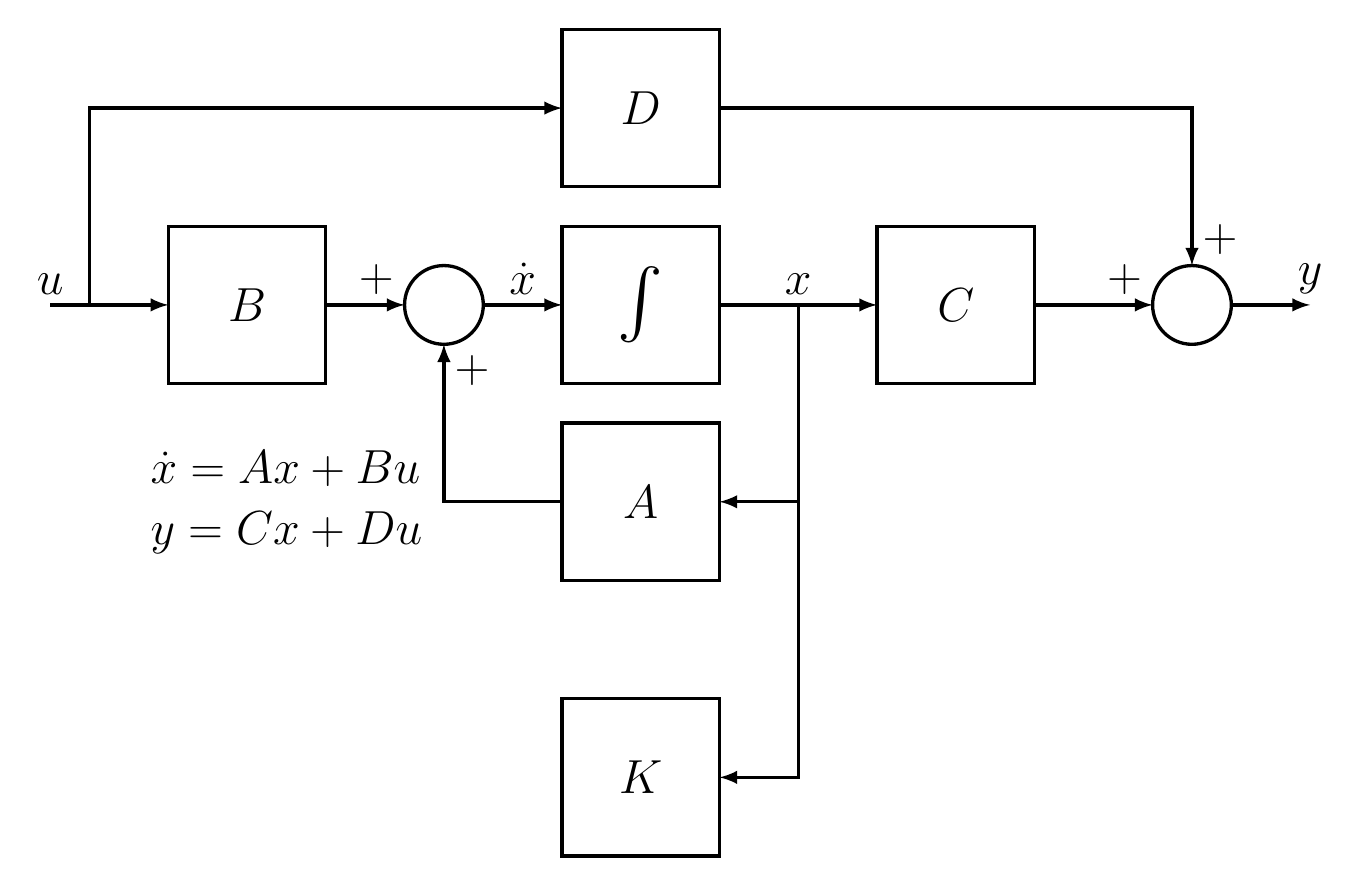
\begin{tikzpicture}[very thick, every node/.style={font=\LARGE}];
      \definecolor{dkg}{rgb}{0,0.5,0};
      % ==========


      \draw (2.5,0) rectangle ++(2,2) coordinate(G)  node[pos=0.5] {\Huge{$\int$}};

      \node at (-1,-1.5) {
        \begin{tabular}{l}
          $\dot{x} = A x + B u$ \\
          $y = C x + D u$
        \end{tabular}
      };

        \draw [-latex, black] (G)++(0,-1) -- ++(1,0) coordinate(X) node[above]{$x$} -- ++(1,0);
        \draw (1,1) coordinate(S) circle (1/2);
        \draw [-latex, black] (S)++(1/2,0) -- ++(1,0) coordinate(E) node[midway, above]{$\dot{x}$};

        \draw (2.5,-2.5) coordinate(A) rectangle ++(2*1,2*1) node[pos=0.5]{$A$};
        \draw [-latex, black] (X) -- ++(0,-2.5) -- ++(-1,0);

        \draw [-latex, black] ($(A)+(0,1)$) -| ($(S)+(0,-0.5)$) node[below right]{$+$};

        \draw (-2.5,0) rectangle ++(2*1,2*1) coordinate(B) node[pos=0.5]{$B$};
        \draw [-latex, black] (B)++(0,-1) -- ++(1,0) node[above left]{$+$};
        \draw [-latex, black] (-4,1) coordinate(u) node[above]{$u$} |- ++(1.5,0);

        \draw (6.5,0) coordinate(C) rectangle ++(2*1,2*1) node[pos=0.5]{$C$};
        \draw (10.5,1) coordinate(y) circle (1/2);
        \draw [-latex, black] (y)++(0.5,0) -- ++(1,0) node[above]{$y$};
        \draw [-latex, black] ($(C)+(2*1,1)$) -- ($(y)+(-0.5,0)$) node[above left]{$+$};

        \draw (2.5,2.5) coordinate(D) rectangle ++(2*1,2*1) coordinate(B)  node[pos=0.5]{$D$};
        \draw [-latex, black] ($(u)+(0.5*1,0)$) |- ($(D)+(0,1)$);
        \draw [-latex, black] ($(D)+(2*1,1)$) -| ($(y)+(0,0.5)$) node[above right]{$+$};

        % State feedback
        \draw (2.5,-6) coordinate(K) rectangle ++(2*1,2*1) coordinate(B)  node[pos=0.5]{$K$};
        \draw [-latex, black] (X) -- ++(0,-6) -- ++(-1,0);
        %\draw [-latex, black] ($(K)+(2*1,1)$) -| ($(y)+(0,0.5)$) node[above right]{$+$};

    \end{tikzpicture}

\end{document}